%  JFL cal section 


\subsection{Aperture photometry NEW}

The calibrators were observed frequently during runs 9 and 10. These observations were beammaps for Uranus and Neptune
as well as  sequences of 4 consecutive
otf maps ($8' \times 5'$) as done for Ceres Vesta, NGC7027, CRL2688, and MWC349. All observations were processed 
to produce intensity maps for the three arrays with the pipeline  in
using kidpar
{\it kidpar-best3files-FXDC0C1-GaussPhot} for the array geometry,
the method {\it COMMON-MODE-ONE-BLOCK}  to remove
 low frequency noise including atmosphere,
sky projection AZEL, line-of-sight opacities, an {\it a priori} mask of $100''$ and no iteration in mapping.
Note that the gain variation with elevation from EMIR implemented in the pipeline has not been used. 
In addition to the fact that they  have flux densities accurately known from models,
Uranus and Neptune are significantly stronger than the other calibrators, and  are the best sources to caracterize the
instrument and calibrate its flux density  scale.

The total flux densities of all observations of Uranus and Neptune during runs 9 and 10 were
measured directly with aperture photometry over a large radius of 150'' to reach saturation level

These measurements are of high quality over a broad range of observing conditions
($33^{\circ}<$ elevations $<58^{\circ}$, and   $0.16 < \tau_{1mm} < 0.50$.
An illustration of our aperture photometry is given in Fig.~\ref{fig:PhAp}.

We emphasize that prior to summation of all the pixels within the aperture, the intensity of each pixel must be estimated
from its brightness  given in Jy/beam in the map provided by the
pipeline (beam stands  for the total beam including beam and side lobes).
The brightness of each pixel must be multiplied by
$dx \times dx / \Omega_{true}$ where  $dx$ is the pixel size ($1''$ in our processing)
and $\Omega_{true}$  is the solid angle of the total beam, traditionally called true.
We have computed the solid angle of the true beam :

$$ \Omega_{true} (r_{max}) = \int_0^{2\pi} \int_0^{r_{max}} B(r) 2 \pi r dr$$

\noindent where $B(r)$ is the radial profile of the azimuthally averaged brigthness over narrow annuli,  $dr$ in width, and normalised so that B(0)=1.
We have used  $r_{max}=250''$ allowed by the size of the maps observed. Only a small fraction of the incident power is
left in side lobes beyond, see Greve et al (1998) and Kramer et al (2013).
This integral is derived from the general expression ({\it e.g.} Adam, 2016, \S 8.1.1.2 of his PhD thesis) for a
brightness distribution assumed azimuthally symmetric.  The excess
of the true beam relative to the Gaussian beam is $\Omega_{true} / 2 \pi (\sigma_{Gauss})^2$, with  $\sigma_{Gauss}$ derived from
the $FWHM$ of each observation. These excesses have been 
estimated  for all observations of Uranus and Neptune in runs 9 and 10 and their histogram are shown
in Fig.~\ref{hist:excesses} (first row of plots). The mean
ratios of solid angles between the true and gaussian beams are
$1.87\pm0.16$  and $1.35\pm0.08$ at 1mm and 2mm, respectively. We note these ratios are consistent with
the beam efficiencies (ratio of powers between main beam  and   total beam)
of $\sim 55$ \% at $\lambda=1$mm ($1/1.87 \times 100$) and $\sim 70$ \% at $\lambda=2$mm ($1/1.35 \times 100$)
found  within the same extent  of $250''$.
The solid angle of the true beam we have determined at each wavelength will be required to convert from
Jy/beam to Jy/pixel or Jy/str. We provide their distribution and mean values in Figure ~\ref{fig:Omega_arcsec2}. 
The solid angle of the total beam is found to be  $\propto \lambda^{\gamma}$ with $\gamma \sim 1$ determined with these mean values
at 1mm and 2mm.  

Finally, we stress again that the gain curve of EMIR, although implemented in the pipeline, was not used for the processing.
We have determined $FWHM$ and $\Omega_{true}$  for each observation, and this
models, at least in part, any change in beam shape with elevation which is usually accounted
for with the gain curve of the telescope. We have further investigated
the excesses $\Omega_{true} / 2 \pi (\sigma_{Gauss})^2$ found in plotting them versus elevation
and attenuation ($exp(-\tau/sin(elev)$) in Fig.~\ref{hist:excesses}.
Over the range covered by the observations between 33$^{\circ}$ and 58$^{\circ}$, there is no correlation
of these ratios with elevation  but  with  attenuation ; these ratios are about 15\% larger at 1mm and 11\%
at 2mm for small attenuation ($exp(-\tau/sin(elev) > 0.8$. This effect is under investigation. 

\begin{figure}
\begin{center}
  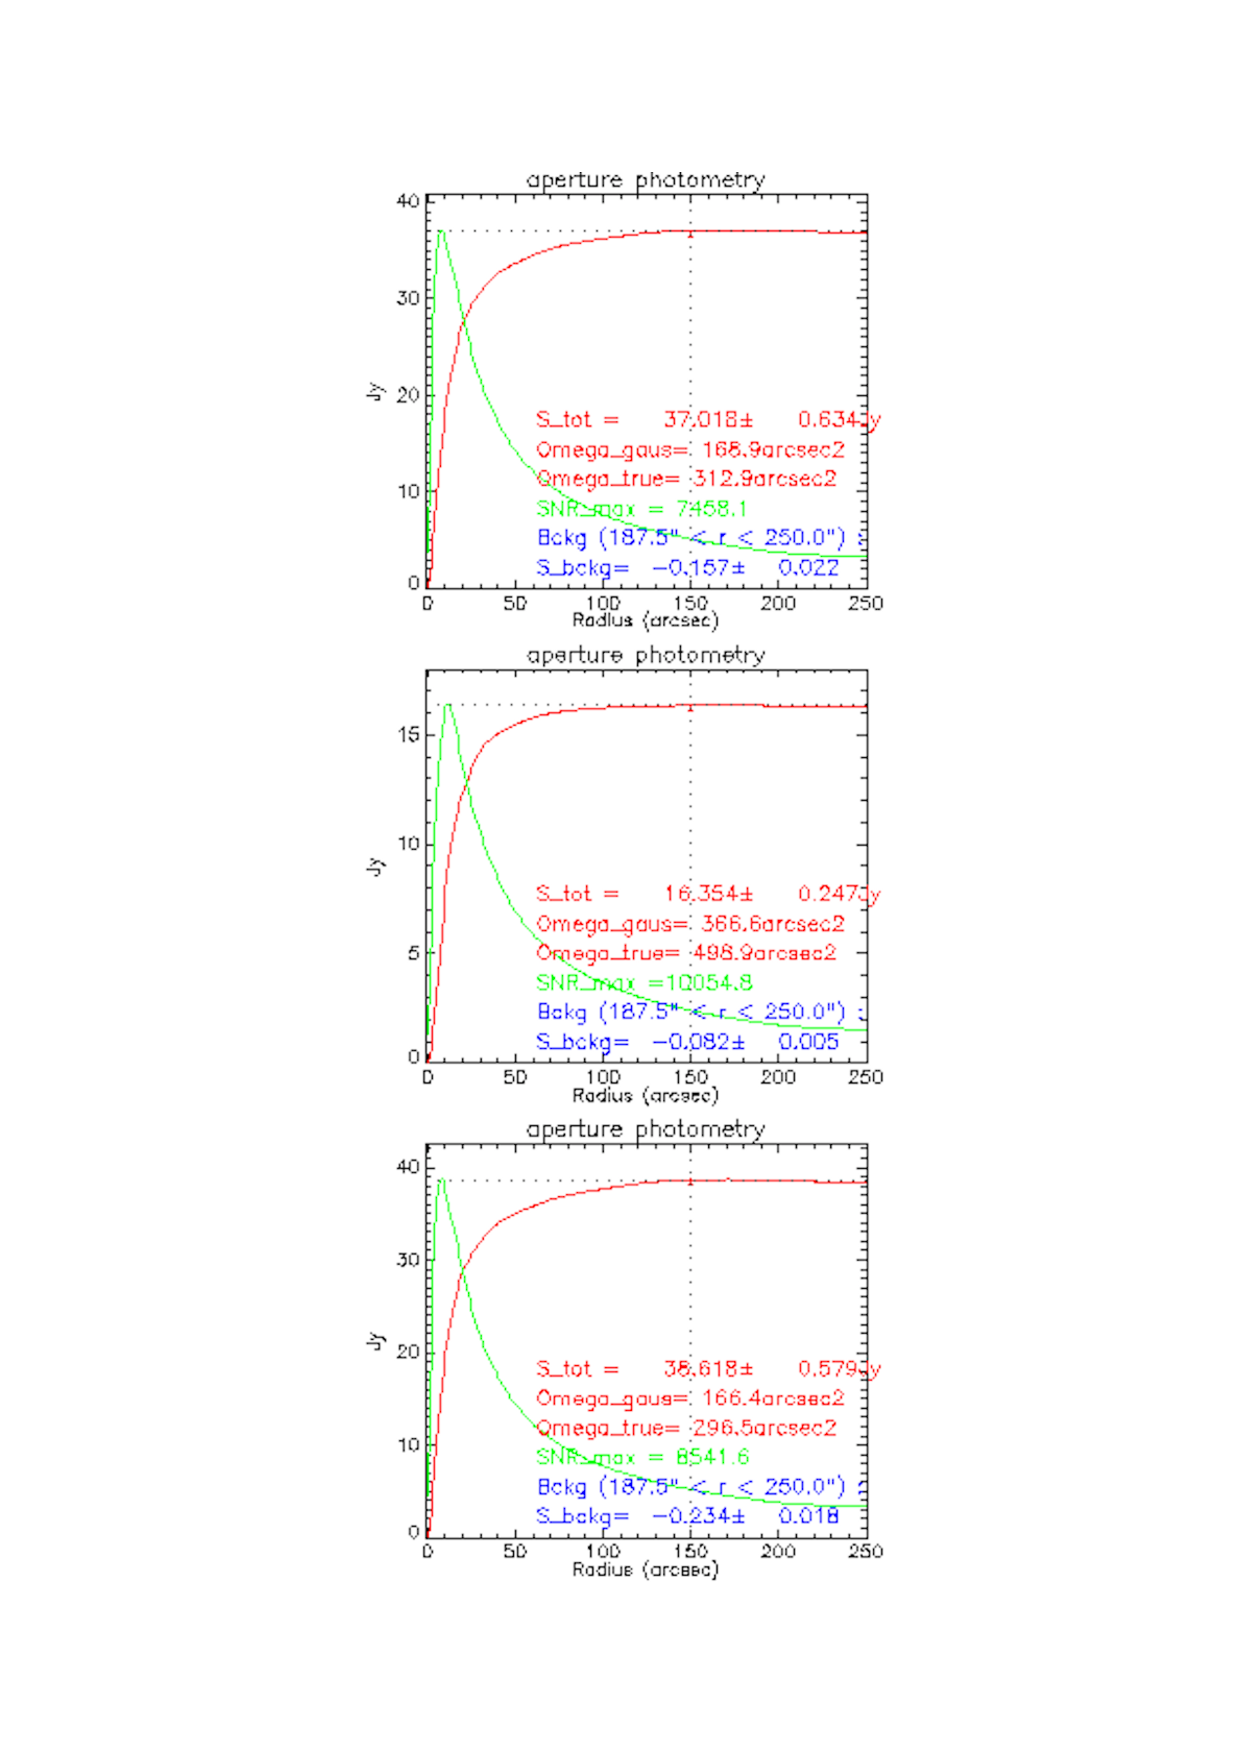
\includegraphics[clip, angle=0, scale=0.4]{Figures/Uranus_s308.pdf}
  \caption{Aperture photometry of Uranus observation 20170227s308  on array 1, 2 and 3 from left to right.
    The photometric curve in red saturates at about the radial distance of  $150''$. (Green curve is the SNR in individual annulus}
\label{fig:PhAp}
\end{center}
\end{figure}






\subsection{Stability of the flux density scale with the primary calibrators Uranus and Neptune }

The inter-run stability of the flux density scale
can be characterised with  the photometry of Uranus and Neptune of run 9 (february 2017) and run 10 (april 2017).
We show the ratios between the measured flux densities
and their reference values at 150 and 260 GHz in Fig.~\ref{fig:U_N_ratio}.  
The resulting mean ratios $\mu$
are close to unity for the three arrays as expected since
the planets were used to set the Jansky scale in average over all the observations early in the processing. It is noticeable
that scatters around unity in Fig. \ref{fig:calibaccuracy}
are about twice smaller in the first session conducted in significantly better weather than during the second session ;
precisely, stabilities for the first session
are 3.6\%, 2.5\% and 2.9\% for arrays 1, 2, 3, respectively, with opacity $\tau_{1mm}$ between 0.05 and 0.3,
and, correspondingly, for the second session, are  5.3\%, 6.7\% and 8.6\%  with  $\tau_{1mm}$ between 0.25 and 0.6.
It is thought, at the moment, that limitations in stability are caused by residual atmospheric fluctuations
in the astronomical signal and uncertainty in opacity corrections.

Nonetheless, the flux density scale of NIKA2 is found to be highly stable and comparable to the level achieved
by other modern instruments, e.g. SCUBA2 (Dempsey, 2013).
The other limitation of the scale is absolute calibration that depends on the
accuracy of the Moreno's model which is estimated to be 5\% in the millimeter wavelength range. Hence, in combining
both limitations,
the total uncertainty of calibration with NIKA2 is $10\%$ in mediocre atmospheric condition and better than $6\%$
in fair condition.

We have plotted the flux density ratios versus elevation, opacity and attenuation in  Fig.\ref{fig:ratio_vs_att} for Uranus and
Neptune. No correlation is apparent. We stress that no gain curve was applied in processing the data but
the solid angle of the total beam (true beam) was determined for each observation. This models any changes
in the beam caused by telescope surface deformation and atmospheric conditions.


Finally, correlations between flux density ratios of the three arrays are shown in Fig.~\ref{fig:U_N_corr}, separately
for runs 9 and  10. Highest correlations are found between arrays 1 and 3.


\begin{figure}
\begin{center}
  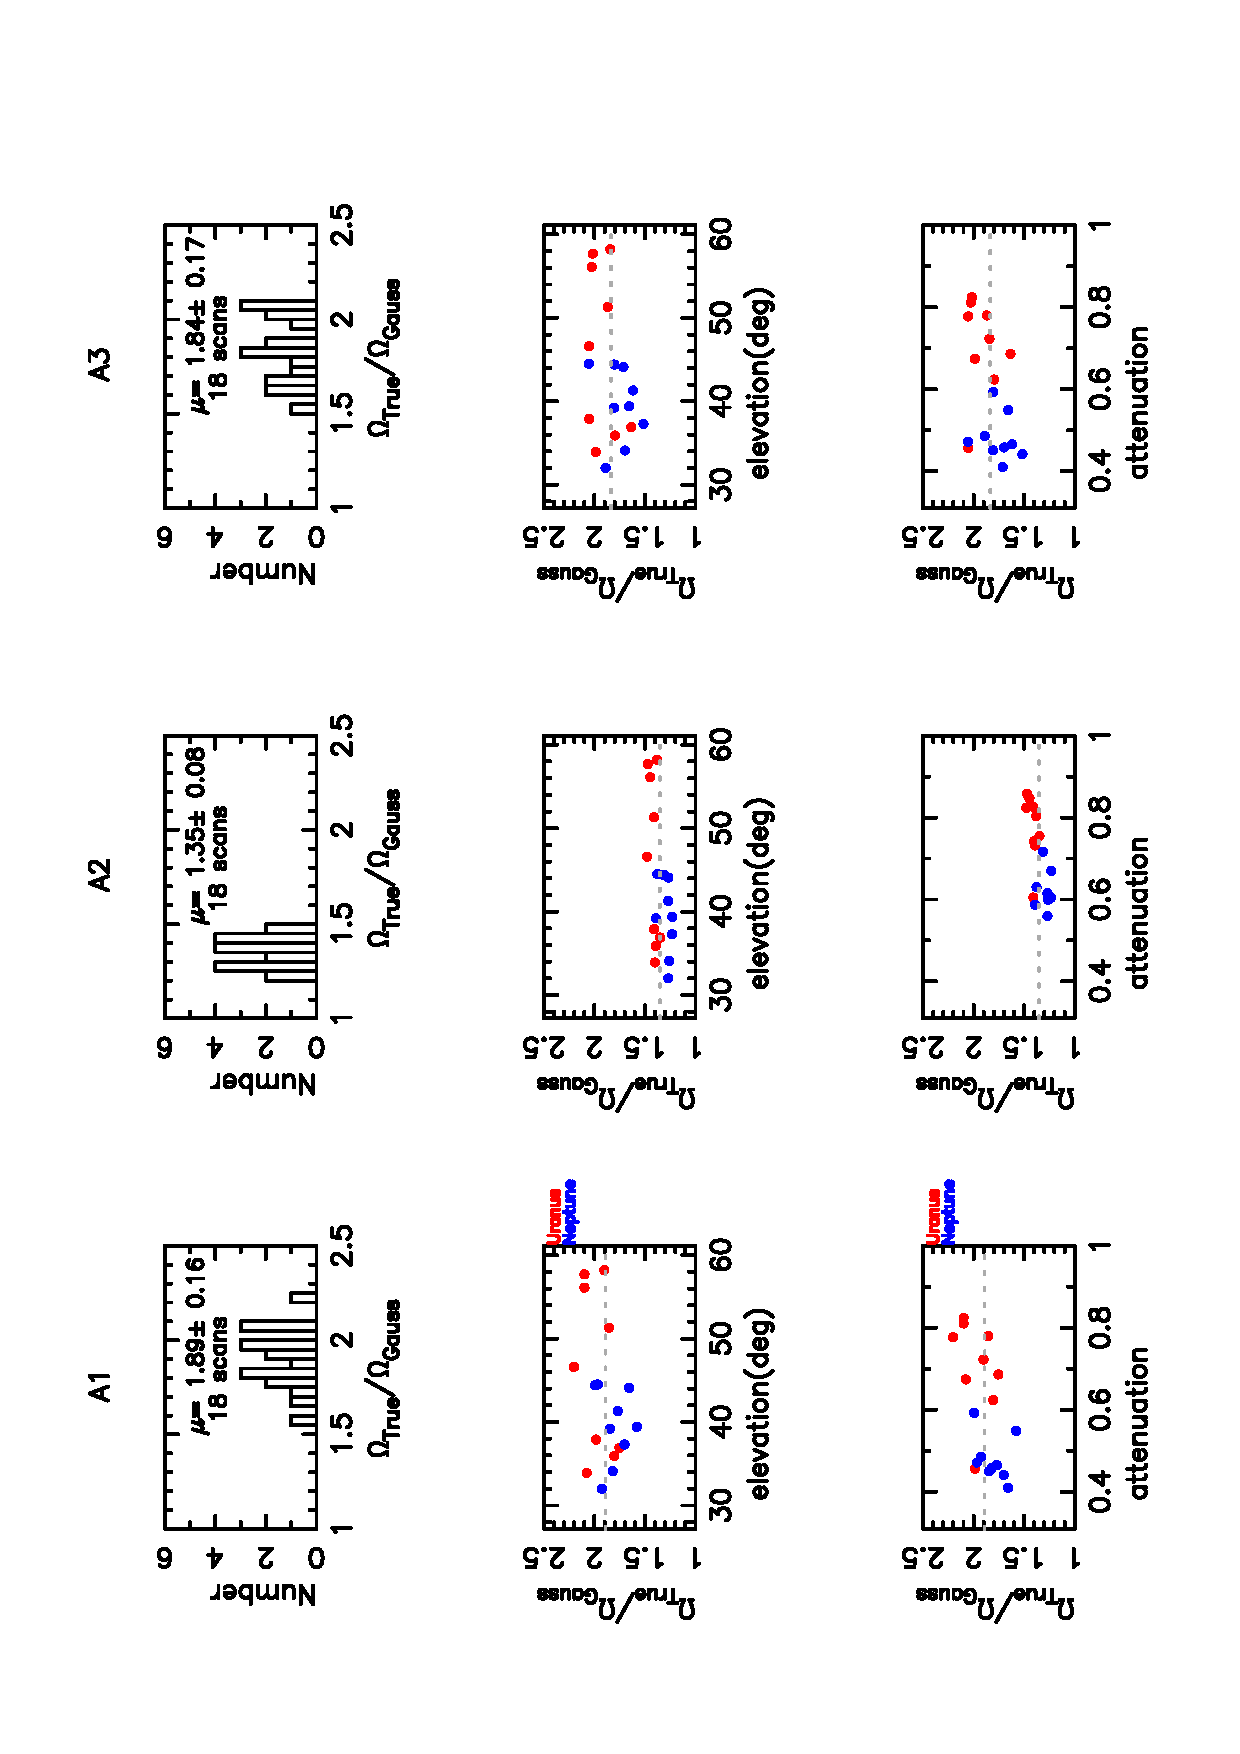
\includegraphics[clip,angle=-90, scale=0.6]{Figures/TG_hist_runs_9_10.pdf}
  \caption{Solid angle excesses between the true and  gaussian beams for all
   observations of Uranus and Neptune during runs 9 and 10.}
\label{hist:excesses}
\end{center}
\end{figure}

\begin{figure}
\begin{center}
  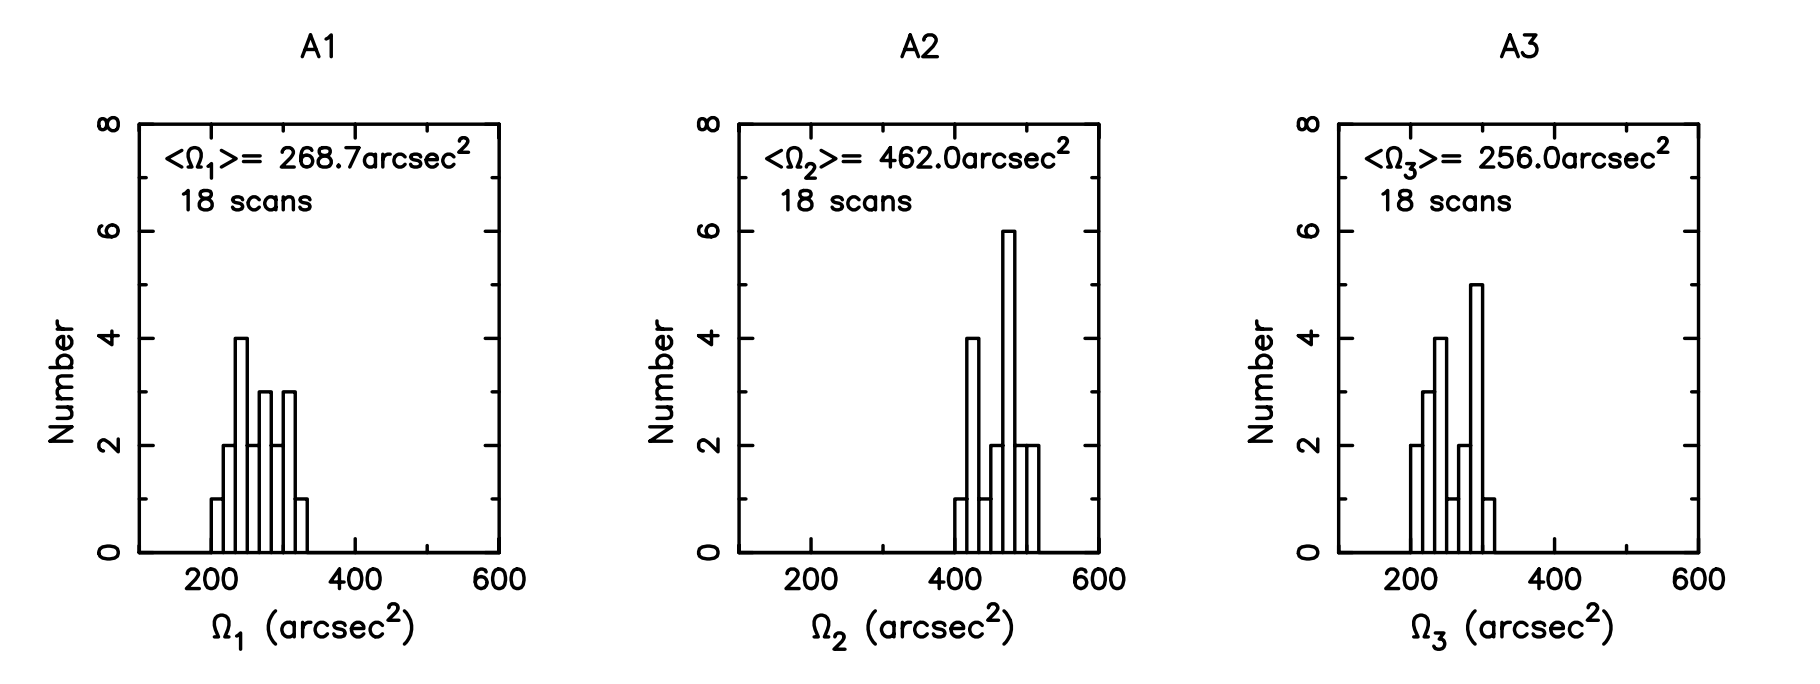
\includegraphics[clip,angle=0, scale=0.5]{Figures/Omega_arcsec2.png}
  \caption{Solid angles of the  true  beams for the three arrays determined
    with Uranus and Neptune during runs 9 and 10. $<\Omega_{1,2,3}>$ in plots are mean values.}
\label{fig:Omega_arcsec2}
\end{center}
\end{figure}




\begin{figure}
\begin{center}
  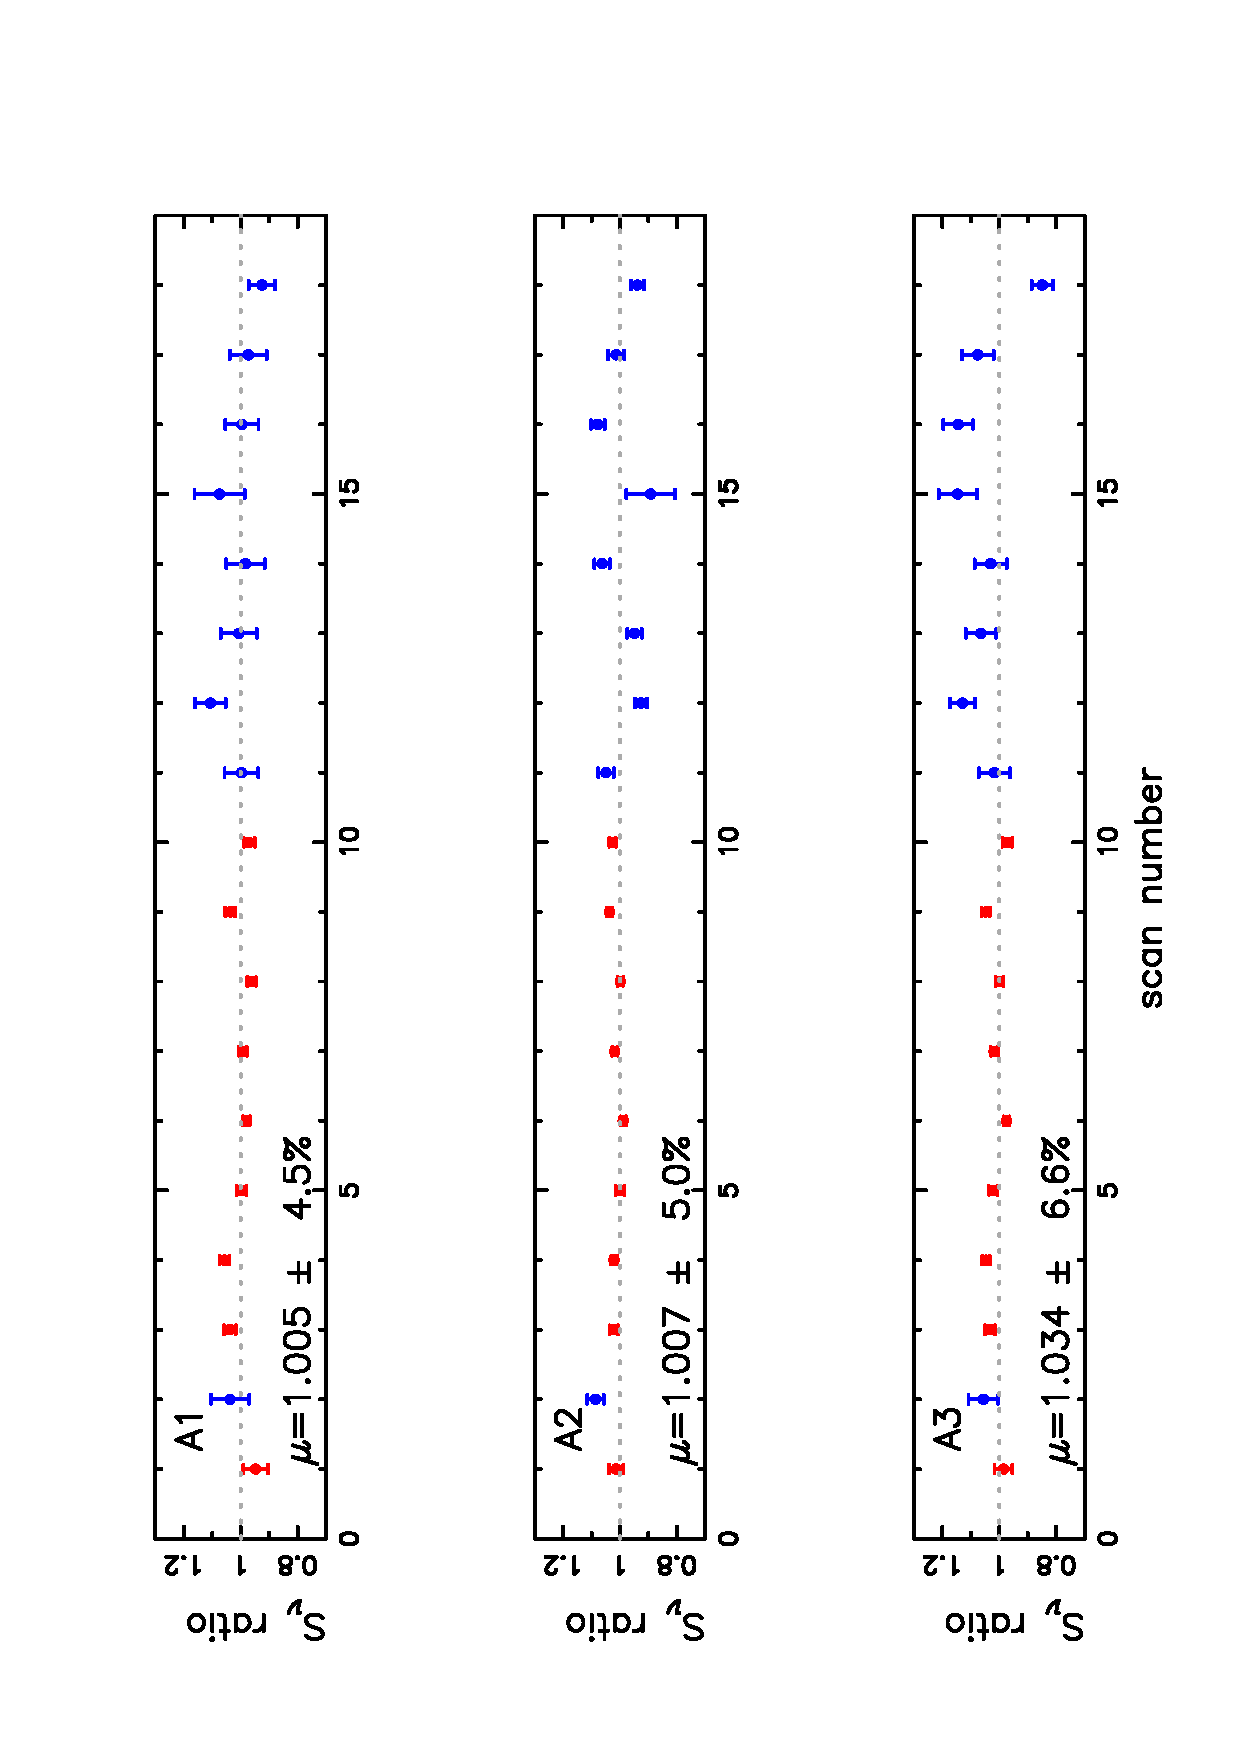
\includegraphics[clip, angle=-90, scale=0.6]{Figures/Ura_Nept_r9_10.pdf}
  \caption{Stability of the flux density scale with the primary calibrators Uranus (red) and Neptune (blue) :
    ratios between their measured and reference flux densities during run 9 and 10.
    Mean ratio $\mu$ and scatter are provided for each array.
    Observation numbers are time ordered : 1 to 10 are 23-28 february 2017 and 11 to 18 are 19-25 april 2017.
    Neptune was hardly visible at the telescope during run 9, and Uranus was not visible during run 10.
    Observations are beammaps (22 minutes) or sequence of 4 consecutive 4 minute long otfs (16 miunutes) that are
    comparable in integration times.}
\label{fig:U_N_ratio}
\end{center}
\end{figure}

\begin{figure}
\begin{center}
  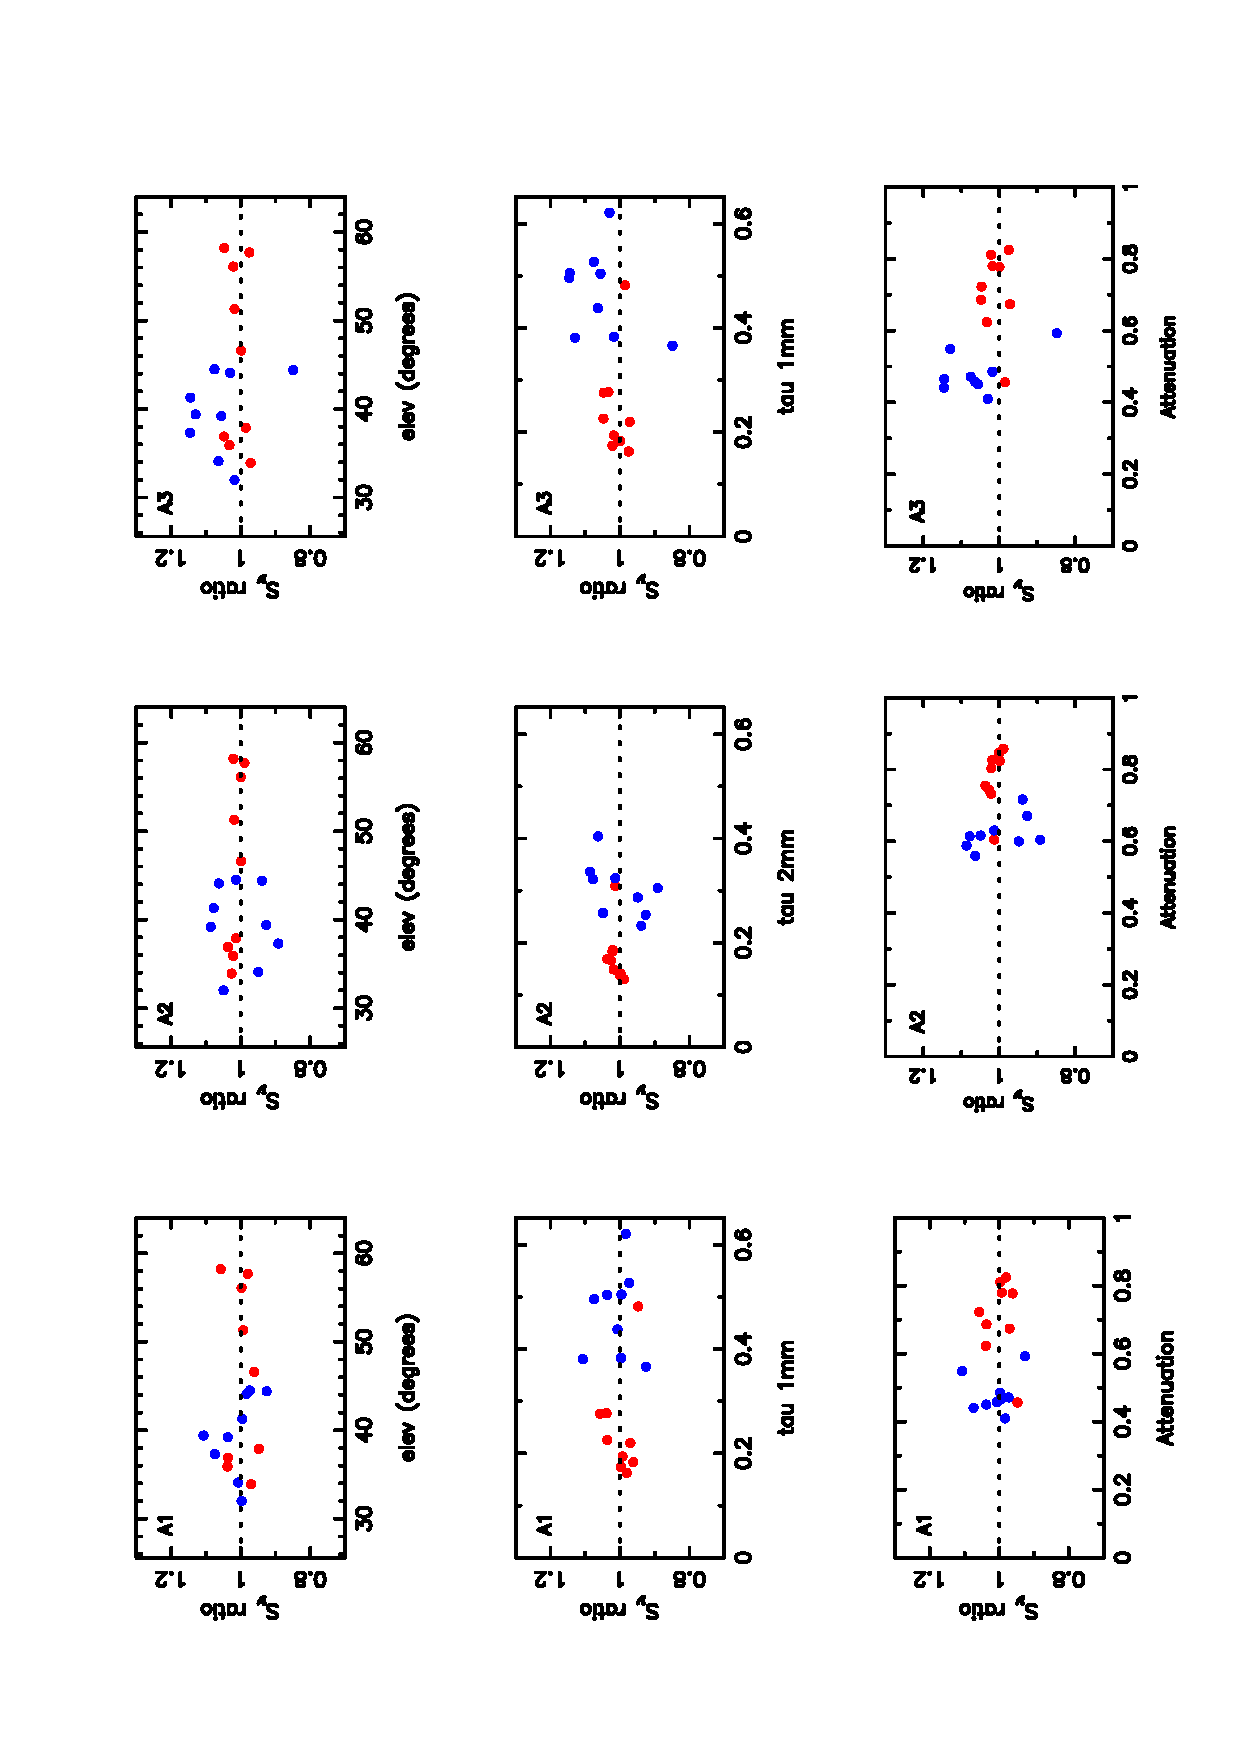
\includegraphics[clip, angle=-90, scale=0.6]{Figures/Ura_Nep_ratio_vs_elev_tau_attenuation_r9_r10.pdf}
  \caption{Flux density ratios versus elevation, opacity, and attenuation ($exp(-\tau/sin(elev)$) for Uranus and Neptune.
    No correlation is apparent with attenuation.}
\label{fig:ratio_vs_att}
\end{center}
\end{figure}


\begin{figure}
%\begin{center}                                                                                                                                               
  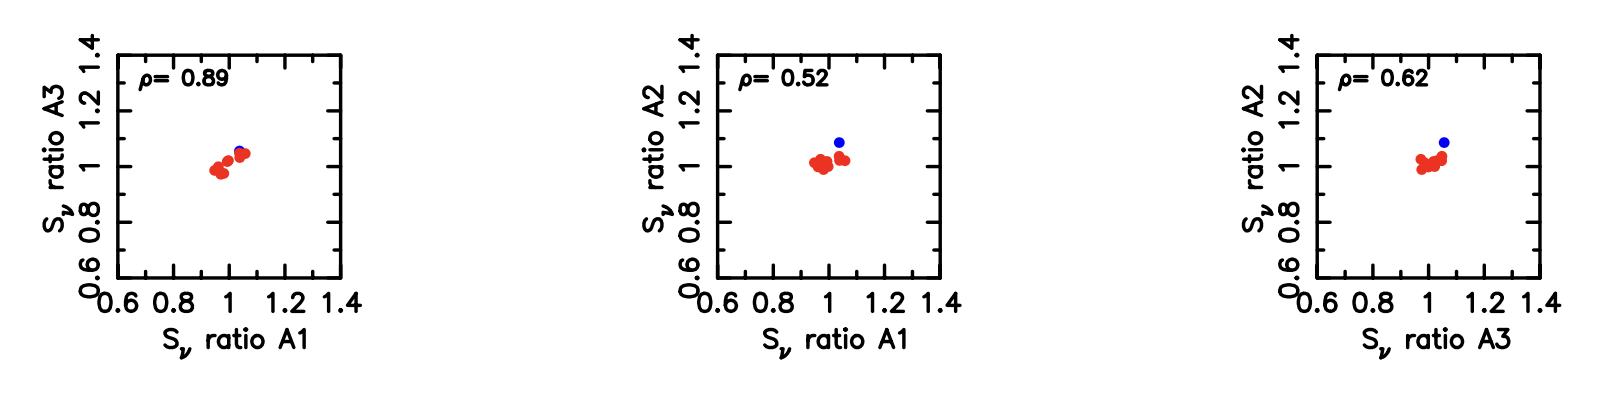
\includegraphics[clip, angle=0, scale=0.55]{Figures/Corr_r9.png}
  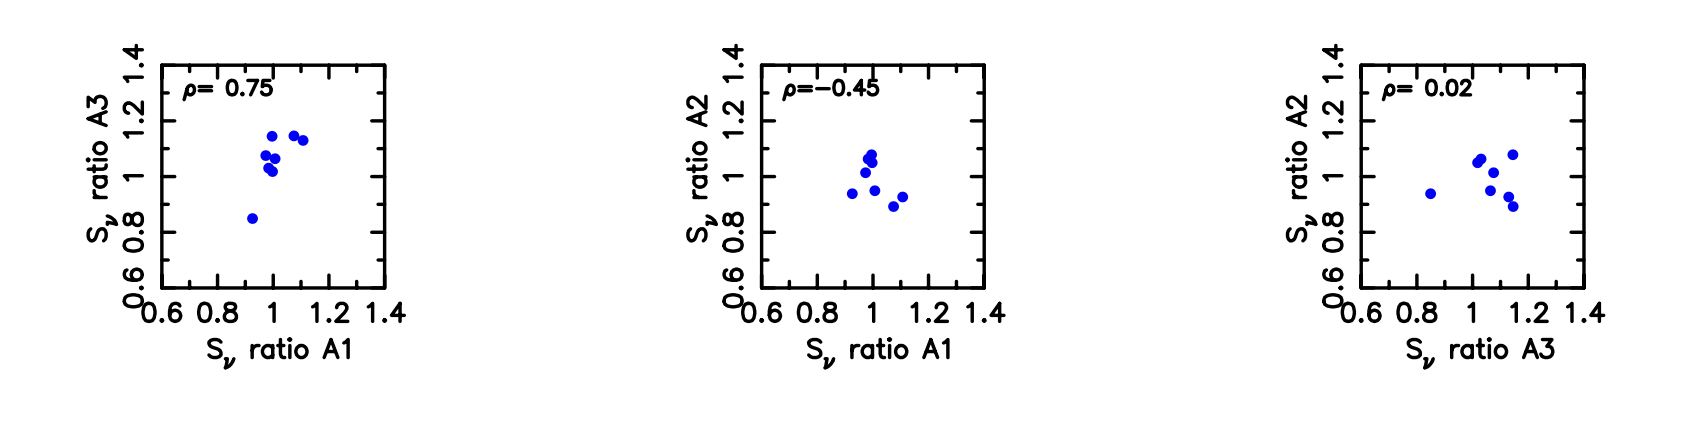
\includegraphics[clip, angle=0, scale=0.55]{Figures/Corr_r10.png}  
  \caption{Correlation plots for the flux density ratios between  the three arrays
    shown separately for run 9 (fair atmospheric condition) and run 10 (mediocre condition).
    Correlation coefficients $\rho$ are given.}
\label{fig:U_N_corr}
%\end{center}                                                                                                                                                 
\end{figure}

\subsection{Stability of the flux density scale with three secondary calibrators }

\begin{table}
\centering
\label{tab:fluxPred}
\caption[]{Reference flux densities of calibrators.}
\begin{tabular}{|l|c|c|c|}
\hline
\multicolumn{1}{|c}{}  & \multicolumn{2}{|c|}{flux  densities (Jy)}  \\
\hline
         &    A1 \& A3  &  A2     \\
         &  260GHz    & 150GHz   \\
\hline
MWC349   &   2.03    &  1.49    \\
NGC7027  &   3.61   &  4.42   \\
CRL2688  &   3.03   &  0.83  \\
\hline
\end{tabular}
\label{tab:flux_cal_sec}
\end{table}

We have extended this  analysis to all the secondary calibrators NGC7027, MWC349, CRL2688
observed during run 9. As for the planets, the observations were processed with the pipeline including line-of-sight opacity.
Aperture photometry was carried out and the solid angle $\Omega_{true}$  estimated from each map.
Four observations of secondary calibrators were discarded because
aperture photometry failed to converge. The remaining 34 observations  provided flux densities on the three
arrays that were compared to their reference flux densities given in Table~\ref{tab:flux_cal_sec}.
Their  ratios  were plotted in Fig.~\ref{fig:ratio_cal_sec} in time order.
All measured flux densities of CRL2688 were too low  at 1mm and 2mm, and its reference flux densities in Table \ref{tab:flux_cal_sec}  had to be decreased
by 10\% at 1mm and 25\%  at 2mm to yield the ratios shown in the Figure. 
All measured flux densities of NGC7027 at 1mm were also too low and its reference flux density had to be decreased by 15\% at 1mm.
All measured flux densities of MWC349 were too high  at 1mm and its reference flux density had to be increased by 5\% at 1mm.

Overall, scatters in the flux density scales of the three arrays with secondary calibrators
are larger than with the stronger planets Uranus and Neptune. They are
14\% for array A1, 7\% for array A2, and 18\% for array A3, during run 9. It is thought that in our treatment with
aperture photometry the solid angle $\Omega_{true}$
estimated from each map is more uncertain because secondary calibrators are fainter than the planets.

We have plotted the flux density ratios versus elevation, opacity and attenuation in  Fig.\ref{fig:corr_cal_sec} for three
secondary calibrator.
A slight correlation with attenuation may be apparent ; flux densities tend to be  10-15\% higher for low attenuation $> 0.8$,
unlike for Uranus and Neptune. It is under investigation.

Color-correction have not been done yet for the secondary calibrators with their spectral indices $\alpha$ different from $\alpha=1.6$ for
the primary calibrators Uranus and Neptune.


\begin{figure}
\begin{center}
  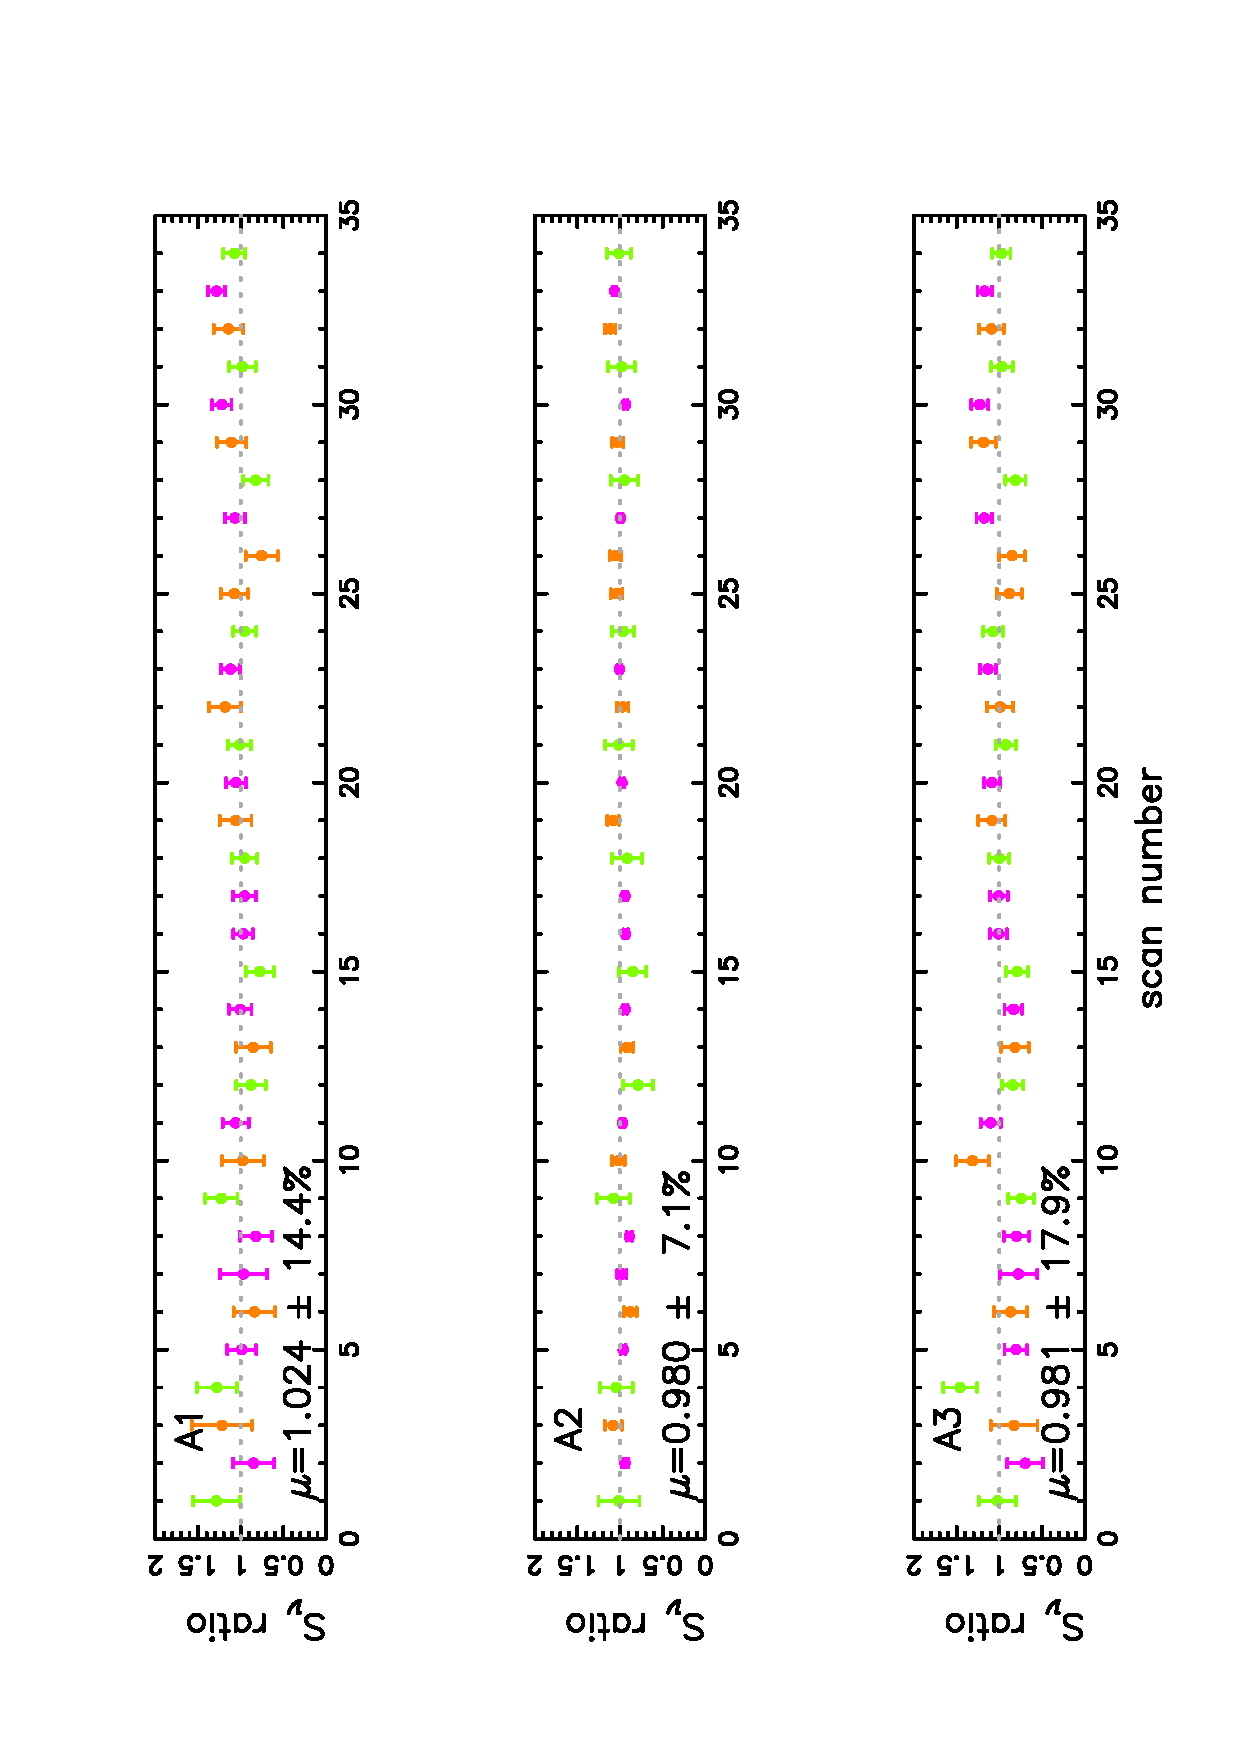
\includegraphics[clip, angle=-90, scale=0.6]{Figures/Flux_vs_index_r9_cal_sec.pdf}
  \caption{Stability of the flux density scale with the secondary calibrators  MWC349 (brown), NGC7027 (purple)  and CRL2688 (green) :
    ratios between their measured and reference flux densities during run 9. Mean ratio $\mu$ and scatter are provided for each array.
    Scan numbers are time ordered. Each observation is a sequence of 4 consecutive 4 minute long otfs (total integration is 16 minutes).}
\label{fig:ratio_cal_sec}
\end{center}
\end{figure}


\begin{figure}
\begin{center}
  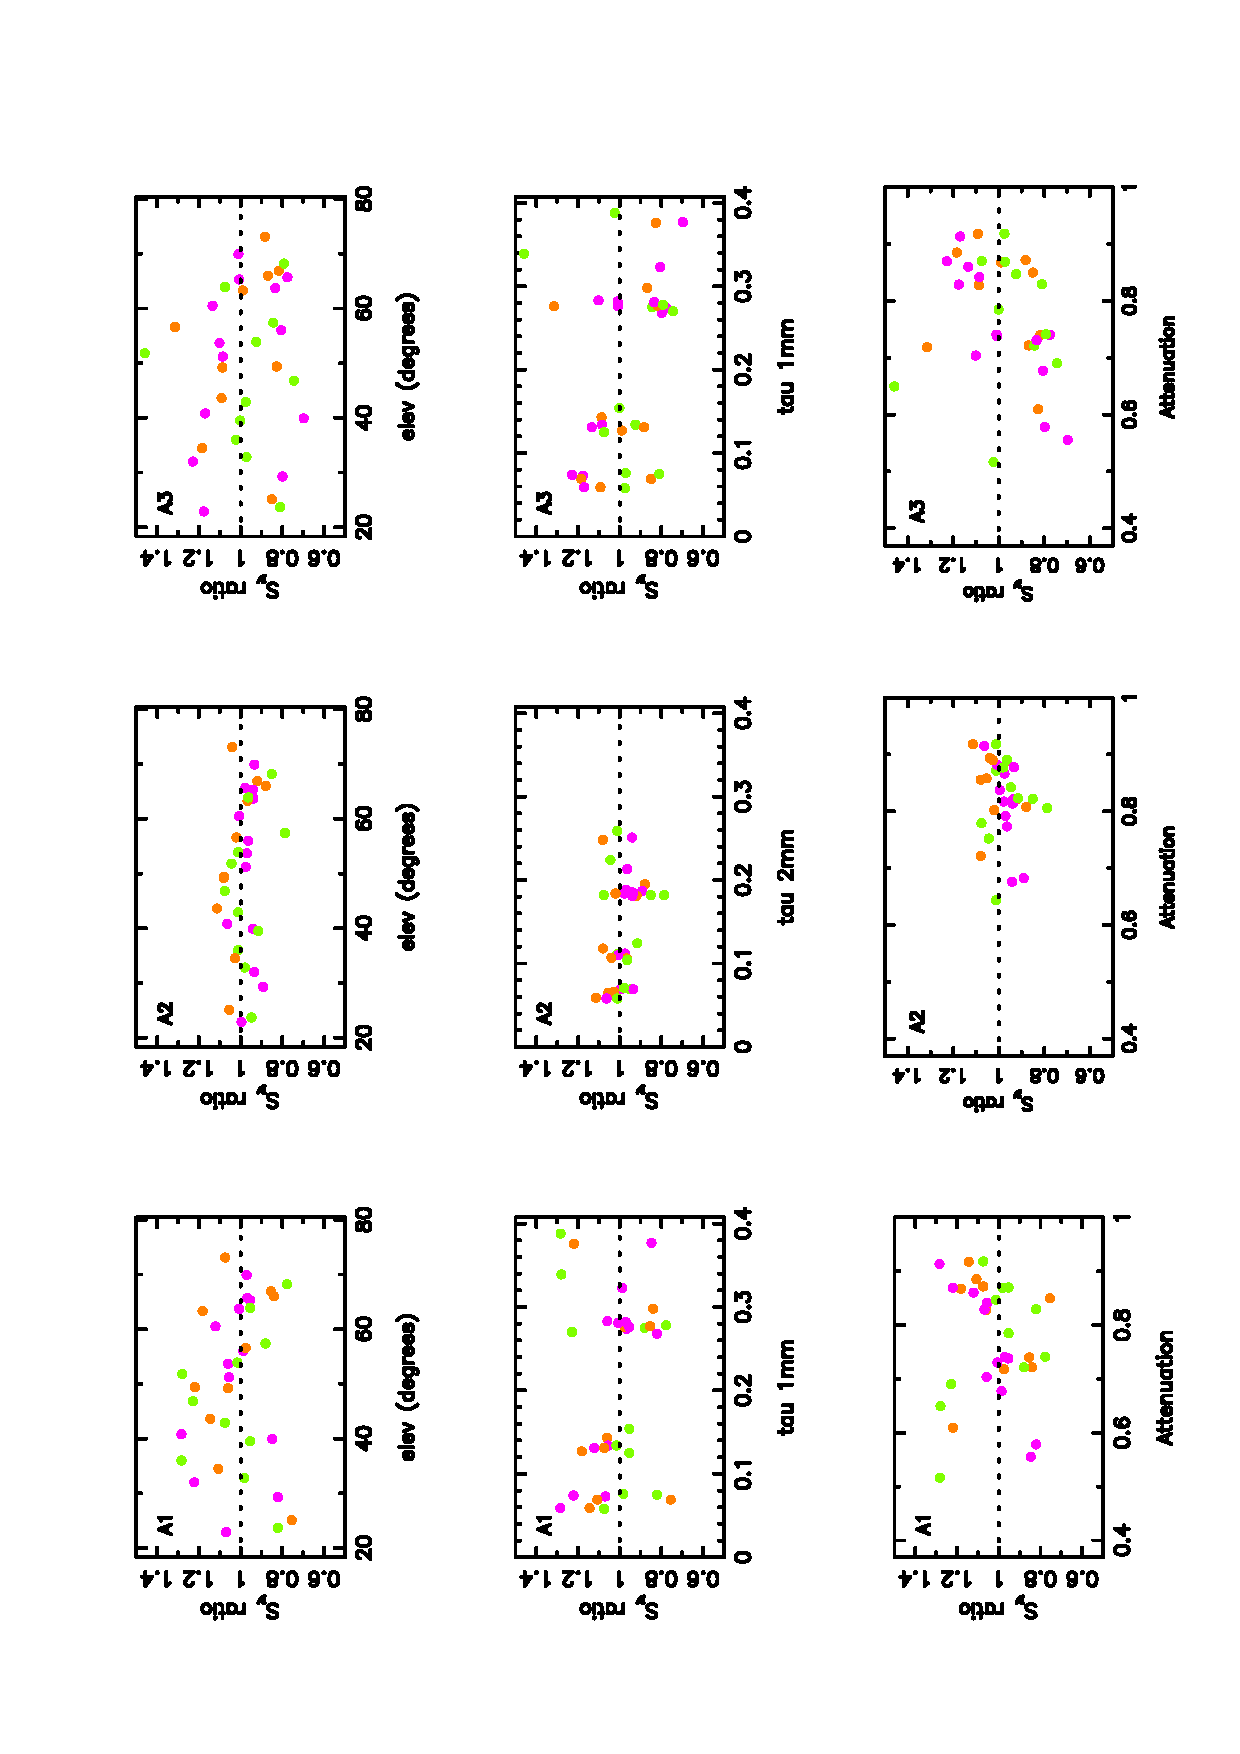
\includegraphics[clip, angle=-90, scale=0.6]{Figures/Ratio_vs_elev_tau_attenuation_r9_cal_sec.pdf}
  \caption{Flux density ratios versus elevation, opacity, and attenuation ($exp(-\tau/sin(elev)$) for the three secondary
    calibrators. A slight correlation 
     with attenuation may be apparent ; flux densities tend to be  10-15\% higher for low attenuation $> 0.8$.}
\label{fig:corr_cal_sec}
\end{center}
\end{figure}

















